\documentclass[a4paper]{article}
\usepackage[T1]{fontenc}
\usepackage[utf8]{inputenc}
\usepackage{lmodern}
\usepackage{amsmath,amssymb}
\usepackage[top=3cm,bottom=2cm,left=2cm,right=2cm]{geometry}
\usepackage{fancyhdr}
\usepackage{esvect}
\usepackage{xcolor}
\usepackage{tikz}\usetikzlibrary{calc}

\parskip 1em\parindent 0pt

\begin{document}

\pagestyle{fancy}
\fancyhf{}
\setlength{\headheight}{15pt}
\fancyhead[L]{Optique}\fancyhead[R]{Question 6}

% Énoncé
\begin{center}
	\large{\boldmath{\textbf{Différence de marche et interfrange \\ pour les trous d’Young}}}
\end{center}

% Correction

\begin{center}
    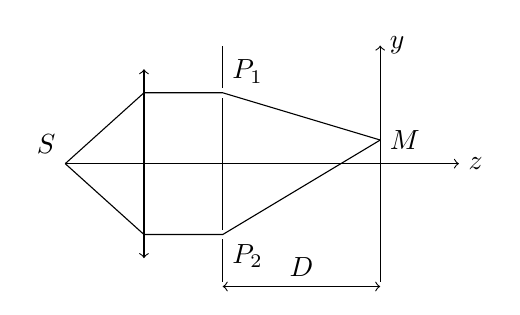
\begin{tikzpicture}[yscale=.6]
        \draw[->] (0,0) node[above left]{$S$} to (5,0) node[right]{$\vv z$};
        \draw[<->] (1,-2) -- (1,2);
        \draw (2,0) -- (2,1.4) (2,1.6) -- (2,2.5);
        \draw (2,0) -- (2,-1.4) (2,-1.6) -- (2,-2.5);
        \draw[->] (4,-2.5) -- (4,2.5) node[right]{$\vv y$};
        \draw (0,0) to (1,1.5) to (2,1.5) node[above right]{$P_1$} to (4,0.5);
        \draw (0,0) to (1,-1.5) to (2,-1.5) node[below right]{$P_2$} to (4,0.5) node[right]{$M$};
        \draw[<->] (2,-2.6) -- node[above]{$D$} ++(2,0);
    \end{tikzpicture}
\end{center}
\par

On a \( \delta = P_2 M - P_1 M\) or \(P_1 M^2 = D^2 + (x - a)^2\) et \(P_2 M^2 = D^2 + (x + a)^2\).\\
On se place proche de l'axe optique avec \( a \ll D \) donc \( (a - x) \ll D \) et \( (a + x) \ll D \).\\
Donc \(P_1 M = D + \dfrac{(x - a)^2}{2D}  \) et \(P_2 M = D + \dfrac{(x + a)^2}{2D}\).\\
D'où \fcolorbox{red}{white}{\( \delta = \dfrac{2ax}{D} \)}\par

Par définition de l'interfrange, \( p(x + i) = p(x) \) d'où \( \dfrac{2a i}{\lambda D} = 1 \)\\
\fcolorbox{red}{white}{Donc \(i = \dfrac{\lambda D}{2a} \)}

\end{document}
